\documentclass[output=paper]{langsci/langscibook} 
\ChapterDOI{10.5281/zenodo.2579039}
\title{Issues in parsing MWEs in an LFG/XLE framework} 

\author{Stella Markantonatou\affiliation{Institute for Language and Speech Processing\slash Athena RIC}\and Niki Samaridi\affiliation{Institute for Language and Speech Processing\slash Athena RIC}\lastand Panagiotis Minos\affiliation{Institute for Language and Speech Processing\slash Athena RIC}}

% \epigram{}

\abstract{We present an LFG/XLE system coupled with an independent lexicographic environment for encoding and parsing Modern Greek MWEs. The system assigns a flat structure to the fixed sequences of words within MWEs, the so-called ``words with spaces" (WWSs) with the help of a preprocessing module that receives the morphologically analysed string from a tagger external to XLE. We describe the overall system and discuss certain implications of the designing choices.}

\begin{document}

\maketitle

\section{Introduction} 
This paper presents the system for parsing \ili{Modern Greek} (MG) Multiword Expressions (MWEs) with \isi{LFG}/XLE grammars that is schematically depicted in Figure~\ref{mar:architecture} and discusses the issues encountered with the \isi{LFG}/XLE representations. The main idea of the adopted parsing strategy is that the parser treats the sequential fixed parts of the MWEs as a type of ``words with spaces” (WWS) \citep{sag02}. Our  WWSs are fixed sequences of fixed words that may contain one word that declines (for instance, see example 7 in Table~\ref{mar:types}). The rigid word order is an important criterion of fixedness in the case of MG that has a relatively \isi{free word order}. Morphological fixedness is also important in a language with rich morphology but, exactly for the same reason, the existence of an inflected word within an otherwise rigid structure is not a surprise. The usage of (this type of) WWSs has practical and theoretical implications. 

WWSs have been used by \cite{copestakeetal2002}, by \cite{attia2006} for parsing \ili{Arabic} MWEs with \isi{LFG} grammars, by \cite{korkontzelosetal2010} for shallow parsing and was recently shown to be beneficial for a transition-based dependency \isi{grammar} parser of \ili{Modern Greek} \citep{apidianaki2018}. We have adopted the WWS approach in an effort to move as much as possible of the parsing burden from the \isi{LFG}/XLE component to an external MWE recognizer (the ``filter'' from now on). At the same time, we have tried to allow for natural \isi{LFG} analyses. 
The system depicted in Figure~\ref{mar:architecture} consists of:
\begin{enumerate}
\item The ILSP FBT Tagger
\item IDION:  A lexicographic tool that allows for formal descriptions of the MWEs 
\item The filter
\item The XLE/\isi{LFG} grammars
\end{enumerate}

\vspace{-.5cm}

\begin{figure}[h!]
  \caption{\label{mar:architecture}The overall structure of the parsing system}
  \centering
  %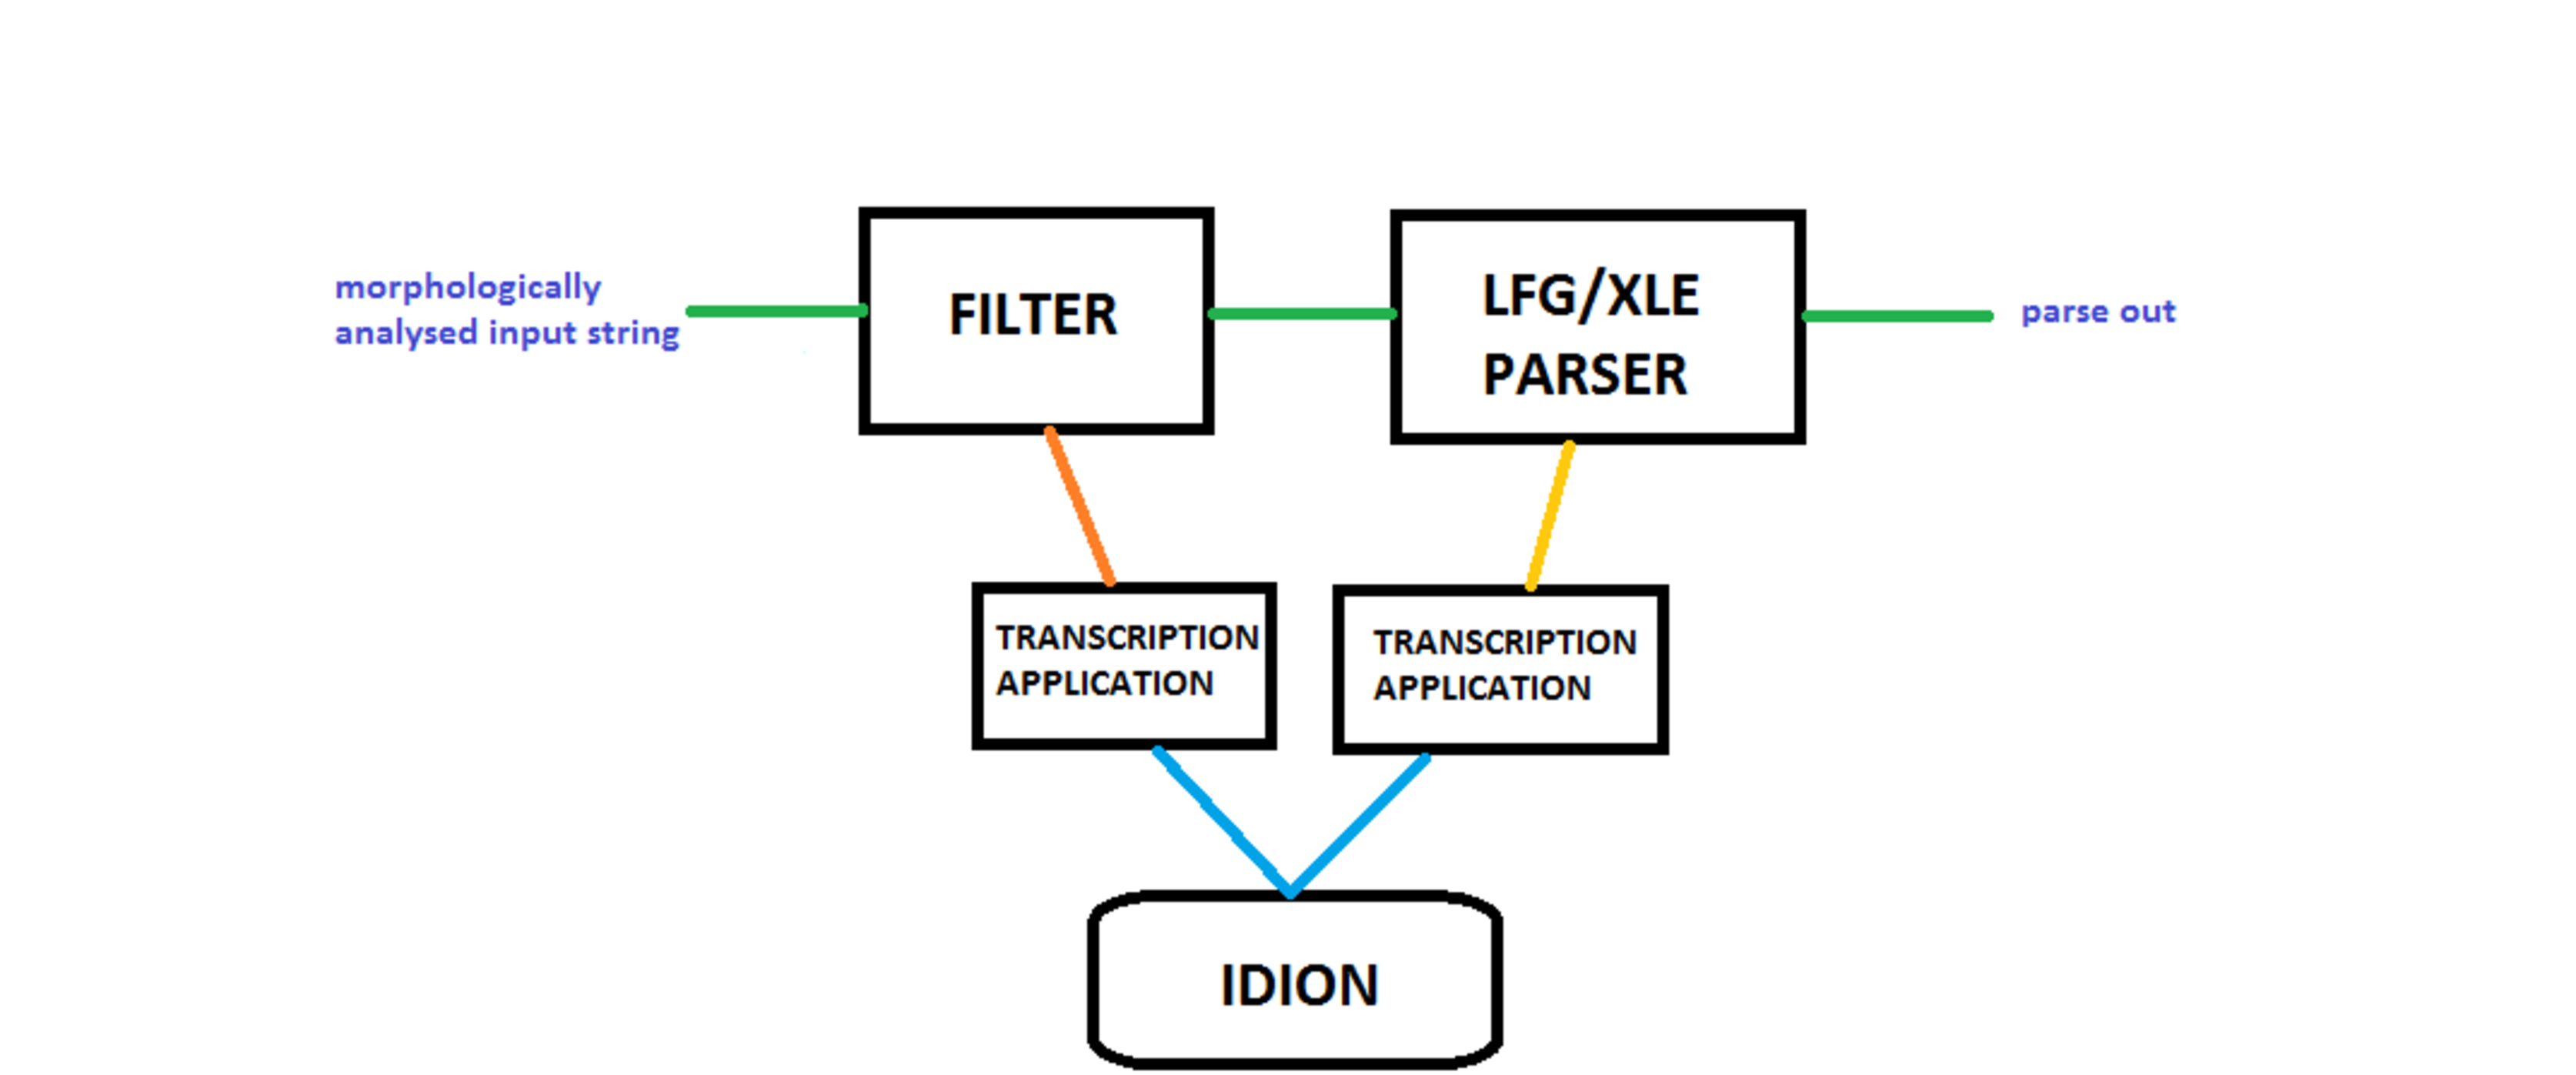
\includegraphics[width=0.99\textwidth]{figures/picture}
  \begin{tikzpicture}[scale=0.68, every node/.style={transform shape}]  
    \tikzset{
      mynode/.style={rectangle, rounded corners, draw=black, top color=white, bottom color=white,very thick, inner sep=1em, minimum size=3em, text width=8em, text centered, font=\bfseries},
      myarrow/.style={->, >=latex', shorten >=1pt, thick},
      mylabel/.style={text width=7em, text centered} 
    }  
    \node[mylabel](morpho) {morphologically analysed input string};
    \node[mynode, right=1.2cm of morpho] (filter) {FILTER};  
    \node[mynode, right=1.2cm of filter] (parser) {LFG/XLE PARSER};  
    \node[mylabel, right=1.2cm of parser](output) {parser output};
    
    \node[mynode, below=1.2cm of filter, xshift=.5cm] (trans1) {{\small TRANSCRIPTION APPLICATION}};  
    \node[mynode, below=1.2cm of filter, xshift=4.5cm] (trans2) {{\small TRANSCRIPTION APPLICATION}};  
    
    \node[mynode, below=1.2cm of trans1, xshift=2.cm] (idion) {IDION};
    
    \draw[myarrow] (morpho.east) -- (filter.west);
    \draw[myarrow] (filter.east) -- (parser.west);
    \draw[myarrow] (parser.east) -- (output.west);
    \draw (filter) -- (trans1);
    \draw (parser) -- (trans2);
    \draw (trans1) -- (idion);
    \draw (trans2) -- (idion);
  \end{tikzpicture} 
\end{figure}

The ILSP FBT Tagger and IDION are independent pieces of NLP software; they are compatible with the ``core" parsing system that consists of the filter and the grammars \citep{samaridi2014}.  In what follows, we describe the parts 1--4 in separate sections in this order. 
We will use (\ref{mar:basicexample}) as a working example. (\ref{mar:basicexample}) is a verb MWE that contains a fixed NP \textit{mavra matia} `black eyes' and an obligatory sentential complement that is controlled by the MWE subject. The subject is free and fully agrees with the verb of the MWE (MG is a pro-drop language therefore in (\ref{mar:basicexample}) no explicit subject is present): 

\ea
\label{mar:basicexample}
\gll kano                  mavra            matia              na do            kapion / kati\\
make.\textsc{1sg} black.\textsc{acc}.\textsc{pl} eye.\textsc{acc}.\textsc{pl} to see.\textsc{1sg}.\textsc{perf} someone {} something\\
\glt `I have not seen someone/something for a long time.’
\z


\section{The LFG analysis adopted: challenging options}
\label{mar:Ssec2}
It has already been stated that the main idea of the adopted parsing strategy is that the fixed parts of the MWEs are treated as “words with spaces” (WWSs) \citep{sag02}.  WWSs are used only if an MWE contains fixed sequences of words; the WWS stands only for the fixed sequence and not for the whole MWE -- if the remaining MWE is flexible. The fixed sequences are identified with diagnostics involving word order permutations, the ability to introduce an XP between words and diathesis alternations (if applicable). As an example, in (\ref{mar:basicexample}) there is the WWS \textit{mavra\_matia} `black eyes'. The sequence \textit{mavra\_matia} is morphologically and syntactically fixed, it can be moved to the beginning of a sentence in emphatic structures and it accepts neither a determiner nor modification. The remaining parts of the MWE in (\ref{mar:basicexample}), with the exception of certain morphological constraints on the subordinated verb, behave like the parts of a compositional structure and are treated as such. 

The \isi{LFG}/XLE lexicon has to recognize the WWSs as words that are assigned some part of speech (PoS) value. However, the selection of the PoS value is not always straightforward with MWEs, all the more when no WWS occurs in the MWE. Examples (\ref{mar:zaxari})--(\ref{mar:psomaki}) illustrate the issue (the identified WWSs are in square brackets ``[]''). We often find nouns functioning as adverbs; in (\ref{mar:zaxari}) the NP headed by \textit{zachari} `sugar' is normally questioned with \textit{how much}. Furthermore, the WWS in (\ref{mar:zaxari}) could be analysed as a syntactic complex, consisting of an  ``object'' clitic and a verb; clitics are used widely in MG.  We treat this complex as a fully inflected verb. The WWS in (\ref{mar:dromous}) could have been generated with the rule NP -> Det  N; given that the head is a common noun (\textit{dromous} `roads') probably the PoS tag ``N'' is a natural choice for the WWS \textit{tous dromous} `the roads'. In (\ref{mar:psomaki}), the WWS is a fixed sequence of fixed words that behaves exactly as the WWS in (\ref{mar:dromous})  with respect to word order phenomena (\hyperref[mar:psomaki]{\ref*{mar:psomaki}a,b}) %\ref{mar:psomakia}-\ref{mar:psomakib})
and unlike the corresponding compositional copula structures of MG (\hyperref[mar:psomaki]{\ref*{mar:psomaki}c,d})%\ref{mar:psomakic}; \ref{mar:psomakid})
. However, there is no \isi{phrase} structure rule that would generate the WWS \textit{to\_psomi\_psomaki} `the bread little-bread' and of course, there is no likely head. 

\ea\label{mar:zaxari}
\gll \textnormal{[}tin             pernao\textnormal{]}  zachari\\
[her.\textsc{acc}.\textsc{fem}   pass.\textsc{1st}]     sugar.\textsc{acc}\\
\glt `I have an easy time.’
\z

\ea\label{mar:dromous}
\gll perno \textnormal{[}tous dromous\textnormal{]}\\
take    [the  roads.\textsc{acc}] \\
\glt      `I wander’
\z

\begin{exe}
\ex \label{mar:psomaki}
\begin{xlist}
\settowidth\jamwidth{(emphatic)}
\ex[]{ \label{mar:psomakia}
\gll leo \textnormal{[}to  psomi  psomaki\textnormal{]} \\
 call [the bread.\textsc{acc}  little-bread.\textsc{acc}]\\
 \glt `to starve’
}
\ex[]{ \label{mar:psomakib}
to psomi psomaki leo \jambox{(emphatic)}
}
\ex[*]{ \label{mar:psomakic}
to psomi leo psomaki \jambox{(emphatic)}
}
\ex[*]{ \label{mar:psomakid}
psomaki leo to psomi \jambox{(emphatic)}
}
\end{xlist}
\end{exe}

      
In addition, the identification of the syntactic function of the fixed parts of verb MWEs is not straightforward in \isi{LFG}. This is so because the governable grammatical functions (GFs) of \isi{LFG}\footnote{The governable GFs of \isi{LFG} are: SUBJ, OBJ, OBJ2, POSS, COMP, XCOMP.} are defined on the basis of particular semantic and syntactic properties \citep{dalrymplelfg}. Alas it is very often the case that the fixed parts of MG MWEs are not characterized by these particular properties. And still, one cannot avoid using a large choice of grammatical functions to model MG MWE phenomena because the language allows for some word order \isi{flexibility} within verbal MWEs (\hyperref[mar:psomaki]{\ref*{mar:psomaki}a,b}) %\ref{mar:psomakia}; \ref{mar:psomakib})
and often there are control (\ref{mar:basicexample}) and binding phenomena (\ref{mar:xronias}) that have to be accounted for. \isi{LFG} models these phenomena on the f-structure with the use of syntactic functions. (In (\ref{mar:xronias}) the WWS \textit{to ksilo tis chronias tis} `the beating the.\textsc{gen} year.\textsc{gen}  hers' can be thought to have a noun head \textit{ksilo} `beating'; the structure contains a possessive pronoun that is bound by the free subject of the MWE.)

\ea\label{mar:xronias}
\gll I Maria             efage  \textnormal{[}to ksilo        tis     chronias       tis    / *tou\textnormal{]}\\
           the Maria.\textsc{fem} ate       [the beating  the    year.\textsc{gen}    hers  / *his]\\
\glt `Maria has been beaten up.'
\z

The OBJ function makes a good example of a \isi{GF} that does not fit well to the MWE data. The WWS \textit{tous\_dromous} `the roads' in (\ref{mar:dromous}) is a fixed simple NP; one would be tempted to assign the OBJ function to it but, on the other hand, the fixed NP never turns up as the subject of a passive form although the verb \textit{perno} `take' passivises. Furthermore, the WWS in (\ref{mar:dromous}) presents an idiosyncratic behavior with clitics; normally it cannot be replaced by a clitic, while this is absolutely possible in a compositional structure; the fixed NP can be replaced only in a very restricted context, namely when the same MWE precedes the structure with the clitic \citep{markantonatou2017} producing an ironic or emphatic effect. Passivisation is a defining property of the OBJ \isi{GF} in \isi{LFG} \citep{dalrymplelfg} and free replacement by a clitic is definitely a defining property of objects in MG. On the other hand, the WWS in (\ref{mar:psomaki}) behaves just as the WWS in (\ref{mar:dromous}) with respect to passivisation and cliticisation and all the other \isi{flexibility} diagnostics; evidence mandates that the two WWSs are assigned the same \isi{GF} and the question is whether they should be assigned the OBJ \isi{GF} or some other \isi{GF}.  It is possible that the idea that MWEs use exactly the syntax employed in the analysis of compositional structures \citep{gross1988a,gross1988b,kay2012,bargmann2017}
could be imported in \isi{LFG} and the classical GFs could be assigned to fixed constituents along with a tree-like structure and constraints on inflection, passivisation, modifiability, cliticisation and linear precedence that do the job \citep{waszczuk2015}. The problem with the  ``compositional structure'' approach is that it questions the notion of syntactic functions and the generalizations expressed with them: for instance, the OBJs of MG MWEs will be peculiar in that they hardly passivise and they are not replaced by clitics freely unless they occur in highly constrained contexts. 

The system we present here uses the classical \isi{LFG} GFs. This means that \textit{zachari} `sugar' in (\ref{mar:zaxari}) is treated as a noun and the phrasal projection is assigned the OBL(ique) \isi{GF}; on the same par, the bracketed strings in (\ref{mar:dromous}), (\ref{mar:psomaki}) and (\ref{mar:xronias}) are assigned the PoS ``No''(un) and project NPs that are assigned the OBJ \isi{GF}. So far we have not used a set of GFs different from the one established in the literature because linear precedence phenomena in the fixed parts are captured with the use of WWSs and modifiability and cliticisation seem to require a more careful modeling than simply allowing or prohibiting them: cliticisation heavily depends on the context and modifiability seems to be rather restricted in MG.  A concrete, corpus-based, analysis of both the phenomena has not been made available yet, to the best of our knowledge. This set-up demands that passivisation is blocked with a feature (and not with the absence of an OBJ \isi{GF} as it would be the case if some other \isi{GF} was used in the place of the OBJ \isi{GF}). Of course, a similar blocking feature would be used in the \isi{grammar} anyway for several non-passivisable transitive verbs of MG MWEs; this fact definitely emphasizes the problematic situation with the OBJ \isi{GF} and passivisation. In a nutshell, we have used the OBJ \isi{GF} not because it served our purposes well but because the in-depth exploration of the alternatives is considered a future challenge.

In the remainder of this document we will present and discuss the parts of the system as they are depicted in Figure~\ref{mar:architecture}. 

\section{ILSP FBT Tagger}
The mature ILSP FBT Tagger \citep{papageorgiou2000} is an adaptation of the Brill tagger trained on MG text. It uses a PAROLE compatible tagset \citep{bilgram-keson:1998:nodalida} of 584 different tags that capture the morphological particularities of MG. The tagger works on the output of a sentence detection and tokenisation tool and assigns both a lemma and a set of tags corresponding to an exhaustive morphological analysis of each token. Figure~\ref{mar:Sfig2} shows the output of the ILSP FBT Tagger for (\ref{mar:basicexample}).
We decided to use the ILSP FBT Tagger because the effort to develop an XFST morphological component is a project on its own. In the set-up of Figure~\ref{mar:architecture}, the tagger is a black box that allows for no identification of the fixed parts of MWEs at the level of morphological analysis, as it would be possible if, for instance, the XFST/XLE component was used as in \cite{attia2006}. For this reason, the morphologically analysed output of the ILSP tagger that offers information only about tokens, is processed with a filter \citep{samaridi2014} that scans the output of the tagger for strings containing MWEs and feeds a script (``formatter'') that transforms the output to a format readable by an \isi{LFG}/XLE \isi{grammar}; the filter informs the XLE parser whether an MWE exists, whether it contains any WWSs -- if so, the WWSs are marked on the output string that feeds the parser -- and whether the input string can receive both a compositional and a MWE interpretation.
\begin{figure}[h!]
  \caption{\label{mar:Sfig2}The output of the ILSP FBT tagger for the verb MWE in (\ref{mar:basicexample})}
  \centering
  %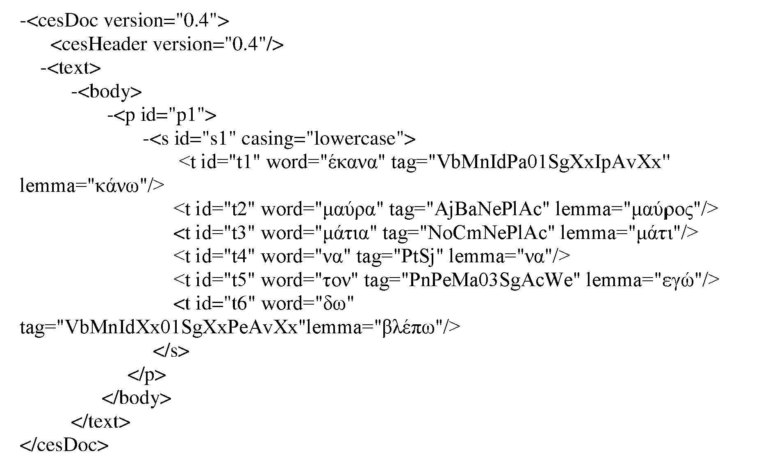
\includegraphics[width=1.\textwidth]{figures/tagger_image1}
\begin{Verbatim}[fontsize=\small]
<cesDoc version="0.4">
  <cesHeader version="0.4"/>
    <text>
      <body>
        <p id="p1">
          <s id="sl" casing="lowercase">
          <t id="t1" word="ἑκανα" tag="VbMnIdPa01SgXxIpAvXx" lemma="κἀνω"/>
          <t id="t " word="μαύρα" tag="AjBaNePlAc" lemma="μαύρος"/>
          <t id="t3" word="μἀτια" tag="NoCmNePlAc" lemma="μἀτι"/>
          <t id="t4" word="να" tag="PtSj" lemma="να"/>
          <t id="t5" word="τον" tag="PnPeMa03SgAcWe" lemma="εγὡ"/>
          <t id="t6" word="δω" tag="VbMnIdXx01SgXxPeAvXx"lemma="βλέπω"/>
        </s>
      </p>
    </body>
  </text>
</cesDoc>
\end{Verbatim}
\end{figure}


\section{IDION}

The XLE parser  receives lexical knowledge on MWEs from IDION\footnote{\url{http://idion.ilsp.gr/}}, an open source lexicographic environment for MWEs that is addressed both to the human user and to NLP applications and encodes, among others, morphosyntactic properties of MWEs in a, as much as possible, theory-neutral formalism. IDION is connected to the parsing system with an application that transcribes the IDION formalism to the XLE formalism \citep{minos2016}.  
As opposed to other MWE DBs, such as DUELME \citep{gregoire:10}, that use a simplified formal language for encoding morphological features, IDION exhaustively describes morphological features with the ILSP-PAROLE compatible tagset that is also used by the ILSP FBT Tagger. 

It is important to note that syntactic functions are assigned to phrasal constituents in \ili{Modern Greek} (and not to parts of a word); therefore, diagnostics for constituent identification are also required along with diagnostics for the identification of WWSs.  In IDION the following diagnostics are used for these purposes \citep{markantonatou2017}: possible word order permutations, the ability of XPs (modifiers included) to intervene between two words thus possibly indicating the border between two constituents, passivisability, clitic replacement, Wh-questioning and causative-inchoative alternations. Grammatical functions are identified with diagnostics that apply to compositional expressions such as morphological marking and Wh-questions (in MG subjects are always in the nominative case and objects almost always in the accusative case, verbs agree with their subjects and objects can be replaced by clitics).

The IDION encoding of the MWE structure corresponds to a rather flat tree and does not make use of powerful expressive means, such as inheritance, that in the literature have been combined with tree-based formalisms \citep{hpsg1,crabbe:etal:13}. The reason for choosing a perhaps redundant but rather simple encoding is that we aim at ensuring IDION's reusability. For this purpose, we try to make sure that we use expressive means that are shared by or can be easily transcribed to many formalisms and that the encoding does not rely on implicit assumptions concerning the overall \isi{grammar} of the language.\footnote{For instance, in MG possession is expressed with the sequence ``DET noun Possessive''. In IDION  the whole sequence is encoded as fixed rather than encoding only the noun as fixed.} To this end, the IDION representation of verbal MWEs defines the following nodes: (i) the root category (default) (ii) the phrasal categories shown in (\ref{mar:idion controlled}) that are used to denote free nominal constituents of the MWE (iii) leaf nodes (words). Phrasal categories and words are directly linked to the root category.  IDION only indexes the fixed contiguous parts of an MWE (the WWSs of our implementation) and does not assign them a phrasal structure.

\ea\label{mar:idion controlled}
NP-NOM/NP-NOM-anim/NP-NOM-nonanim;\\ 
NP-GEN/NP-GEN-anim/NP-GEN-nonanim;\\ 
      NP-ACC/NP-ACC-anim/NP-ACC-nonanim; \\
\z

The Java-based transcription application provides for the remaining phrasal categories needed for an \isi{LFG} representation that requires the definition of constituents and typically involves trees deeper than the ones defined in IDION. 
All in all, IDION only specifies the phrasal categories shown in  (\ref{mar:idion controlled}) and it is on the transcription applications to specify the categories that are necessary for any given formalism.

 The IDION encoding of the MWE in (\ref{mar:basicexample}) is given in Figure~\ref{mar:Sfig3}. On the first column it is specified whether the annotated part of the MWE is a phrasal category (phrasal categories are shown in [\ref{mar:idion controlled}]) or a word and whether it is optional or not (for instance, the MWE of example (\ref{mar:basicexample}) that is depicted in Figure~\ref{mar:Sfig3} has only obligatory parts). Words are encoded as lemmas and only complementisers are encoded as such (in Figure~\ref{mar:Sfig3}, the depicted MWE contains a complementiser).  On the second column, the lemmas of the parts of the expression are listed, namely the verb head \textit{kano} `make', the lemmatized parts of the WWS \textit{mavros mati} `black eye', the complementizer \textit{na} `to' that always  introduces a sentential complement and the lemma form of the irregular verb head \textit{vlepo} `see' of the sentential complement. On the third column are encoded the actual form of the WWS and the control facts; in the case depicted in Figure~\ref{mar:Sfig3},  the sentential complement is controlled by the NP-NOM-anim. The fourth column provides the full morphological analysis of the fixed or semi-fixed parts of the MWE, for instance it is specified that the head verb of the controlled sentential complement is always in the active voice and in a form denoting perfect aspect; person and number of the controlled verb are not specified as they are determined by the free subject of the MWE. On the last column the parts of the WWS are indexed. 

 \begin{figure}[h!]
  \caption{\label{mar:Sfig3}The IDION encoding of the MWE in (1)}
  \centering
 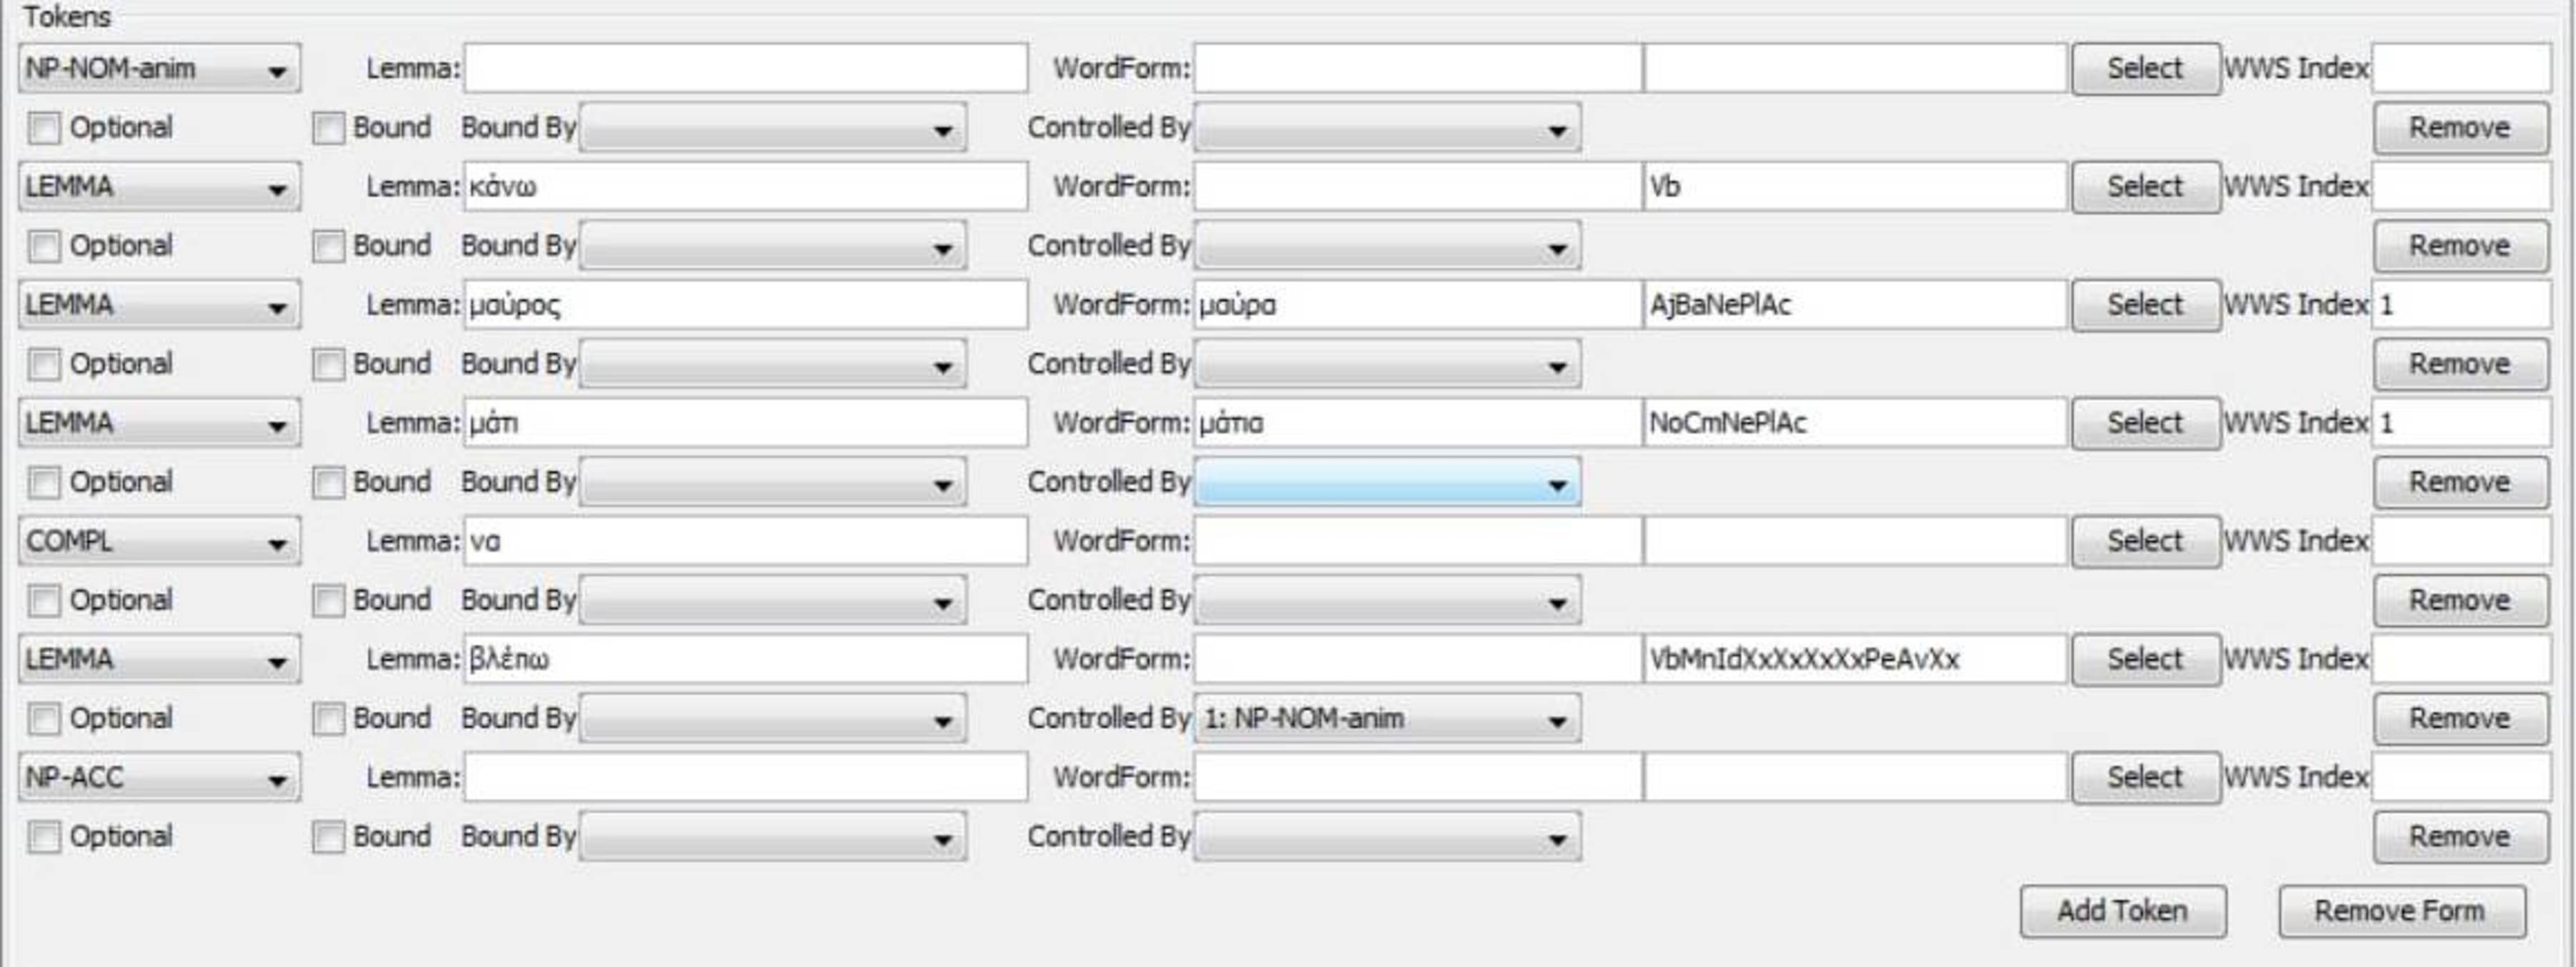
\includegraphics[width=1\textwidth]{figures/idionencoding}
\end{figure}
 



We developed a Java transcription application that generates XLE entries from the IDION specifications. 

The \isi{LFG}/XLE entries listed below are developed out of the IDION representation of (\ref{mar:basicexample}) shown in Figure~\ref{mar:Sfig3}. As a first step, the transcription application generates lexical entries for the WWSs that are indexed in the IDION representation of the MWE;  if one or more WWSs have been indexed in the IDION representation of the MWE, a corresponding number of XLE entries are produced and stored in the XLE lexicon. Morphological information about the entries, here the WWS and the verb head of the controlled sentential complement, is received from the annotation encoded on the fourth column. Next, the application generates the entry for the head verb of the MWE as follows: the NP-NOM-anim slot in the first column shows that the verb selects a free subject NP, the WWS that contains a noun and an adjective both in the accusative case shows that the head verb selects a fixed object and finally,  the existence of a COMPL(ementiser) slot in the first column coupled with the control information on the third column shows that the head verb subcategorises for an XCOMP controlled by the subject of the main verb.  This information generates the entry of the head verb \textit{kano}.  Finally, the head verb of the sentential complement is retrieved from the second column as it immediately follows COMPL. The application knows that the verb \textit{vlepo} is transitive because it has a controlled subject and it is followed by an NP-ACC. \\

%\clearpage

\noindent
The WWS in MWE (\ref{mar:basicexample}): %\\
~\hspace*{1em}mavra\_matia, NoCmPlAc \\

\noindent
The verb head of MWE (\ref{mar:basicexample}): %\\
~\hspace*{1em}kano<SUBJ,OBJ,XCOMP>\\
~\hspace*{15em}$\uparrow$ OBJ PRED = mavra matia\\
~\hspace*{15em}$\uparrow$ XCOMP PRED = vlepo<SUBJ,OBJ>\\
~\hspace*{15em}$\uparrow$ XCOMP PRED FINITE = +\\
~\hspace*{15em}$\uparrow$ XCOMP SUBJ= $\uparrow$SUBJ\\

\section{The filter}
Τhe filter consists of two parts: the filter lexicon and the filtering part proper. 

\subsection{The filter lexicon}
The filter consults the filter lexicon where each MWE entry is specified for the following:

\begin{enumerate}
\item Compositionality: Certain MWEs can take a compositional interpretation. For instance, the free subject verbal MWE in (\ref{mar:basicexample}) has no compositional interpretation while the semi-fixed MWE in (\ref{mar:tis arpazo}) can also take the compositional interpretation `I grab them.\textsc{fem}’. 

\ea\label{mar:tis arpazo}
\gll tis                  arpazo\\
them.\textsc{fem} grab.\textsc{1sg}\\
\glt `I am beaten up.’
\z

\item The ‘signifier’: the lemma of the substring of an MWE that instructs the filter to look at the appropriate filter lexicon entries. For the MWE in (\ref{mar:basicexample}), the signifier is the lemma \textit{kano} `make, do'. If the expression is fixed as in (\ref{mar:perno pente}) the symbol ``\textasciitilde{}'' is used as a signifier.  (\ref{mar:perno pente}) has no translation, it is a kind of swearing (often accompanied with an offensive gesture) meaning that someone has made a serious mistake or is totally idiot:
  
 \ea\label{mar:perno pente}
\gll pare pente\\
take.\textsc{2sg}.\textsc{imp} five\\ 
%\glt `I am beaten up.’
\z

\item The lemmatised form of  ``words with spaces'' (WWSs) whether they are independent fixed MWEs as in (\ref{mar:perno pente}) or substrings of an MWE as in (\ref{mar:basicexample}). In the case of (\ref{mar:perno pente}) the lemmatised WWS would be \textit{perno pente} `take five'. In the case of (\ref{mar:basicexample}) the fixed part is \textit{mavra matia} `black eyes' and the corresponding lemmatised form is \textit{mavros mati} `black eye'.\\

\item PoS and morphological constraints on the parts of the WWS. For the fixed part of (1) \textit{mavra matia} the constraints would be: \textit{mavros}: adjective, plural, accusative, basic; \textit{mati}: noun, common, plural, accusative. 
\end{enumerate}

\subsection{The filtering part}
The filter proper, implemented in Perl, reads the tagged sentence from an \textsc{XML} file (the output of the tagger) and stores it. Then, it checks whether a signifier exists and, \\
\begin{enumerate}
\item[A1.] If no signifier is found, the string is copied as it is on the formatter. 
\item[A2.] If a signifier is found, the filter lexicon is scanned for some WWS entry. The filter checks whether the morphological constraints on the filter lexicon entries (headword and remaining words) match the lemma and the tags on the input string and:
\item[B1.] If they do not match, the input string is copied as it is on the formatter.
\item[B2.] If they match, the filter consults the filter lexicon whether the MWE can take a compositional reading and, 
\item[C1.] if it can, it sends to the formatter the input string and goes to step C2
\item[C2.] if it cannot, the part of the string that has been recognized is replaced with the corresponding WWS and morphological constraints and the resulting new string is sent to the formatter.
\end{enumerate}

\section{The LFG analysis (implemented with XLE grammars)}
The output of the formatter is processed with an \isi{LFG} \isi{grammar} of \ili{Modern Greek} with sub-lexical rules that can parse the output of the tagger. The \isi{grammar} runs on XLE, a parsing environment dedicated to writing, running and debugging \isi{LFG} grammars.\footnote{XLE is the basis for the Parallel Grammar Project, which is developing industrial-strength grammars for \ili{English}, \ili{French}, \ili{German}, \ili{Norwegian}, Japanese, and Urdu. XLE is written in C and uses Tcl/Tk for the user interface. It currently runs on Solaris Unix, Linux, and Mac OS X.} The trees generated by the sub-lexical rules can be seen in the c-structure of Figure~\ref{mar:Sfig6}. 

\ili{Modern Greek} verbal MWEs are rich in \isi{syntactic structure} despite any simplifications that might result from the usage of WWSs. In Section~\ref{mar:Ssec2} we discussed why we have adopted an \isi{LFG} analysis that applies the classical \isi{LFG} Grammatical Functions on MWEs despite the obvious problems. Thus, so far we have manipulated the lexicon by introducing the idiomatic lexical entries but we have not manipulated the \isi{grammar} rules.

With the reservations discussed in Section~\ref{mar:Ssec2} in mind, we proceed to present Table~\ref{mar:types} where the various types of parsed MWE structures are listed. In all, simple sentences containing 850 verb MWEs have been parsed. In Table~\ref{mar:types} we give the basic form of the MWEs: the reader should keep in mind that MG is a pro-drop language with no infinitives, therefore the 1st person singular present indicative (or the 3rd person present indicative if the verb is an impersonal one) are used as the verb's lemma. Our system parses strings in the Greek alphabet but in Table~\ref{mar:types} we have used Latin characters for reasons of readability. We represent WWSs as sequences of words joined with underscores, e.g. \emph{pare\_pente} (\textbf{1} in Table~\ref{mar:types} and example [\ref{mar:perno pente}]). The column headed with ``C'' indicates whether the MWE receives a compositional interpretation (Y) or not (N). Lastly, the column headed with ``FX'' shows whether the MWE is flexible (FL), semi-flexible (SF) or fixed (F). We have marked as SF the MWEs that allow for no word order permutations but their head verb declines fully. MWEs that allow for word order permutations and their head verb declines fully are marked as FL.

With the approach described here, the lexicon has to be enriched with verb-like predicates such as \emph{ego\_arpazo} (\textbf{2} in Table~\ref{mar:types}) and \emph{piano\_gematos} (\textbf{9} in Table~\ref{mar:types}), noun-like predicates such as \emph{mavros\_mati} (\textbf{10} in Table~\ref{mar:types}) and adjective-like predicates such as \emph{tapi\_ke\_psichremos} (\textbf{7} in Table~\ref{mar:types}) and their morphological para\-digms. Therefore, the morphological paradigm of the verb \textit{arpazo} has to be duplicated in order to develop the paradigm of \emph{tis\_arpazo}. Similarly,  (\textbf{7} in Table~\ref{mar:types}) \emph{meno tapi\_ke\_psichremos} contains a WWS that consists of the cranberry word \textit{tapi}, the conjunction \textit{ke} `and' and a fully declinable adjective \textit{psichremos} `cool' that occurs freely in compositional structures. However, the overall amount of new lexical entries is not more than the entries required when MWEs are parsed like compositional structures (that is, without assuming WWSs) because in a ``compositional approach'' the same number of entries (or more) would be listed as ``idiomatic''. We have already pointed out that if the presented system is provided with the appropriate lexical entries and their morphological paradigms, it uses the \isi{grammar} developed for compositional structures to parse sentences containing verb MWEs. 

\begin{table}[htbp]
\caption{\label{mar:types}Types of MG verb MWEs}
\centering
%%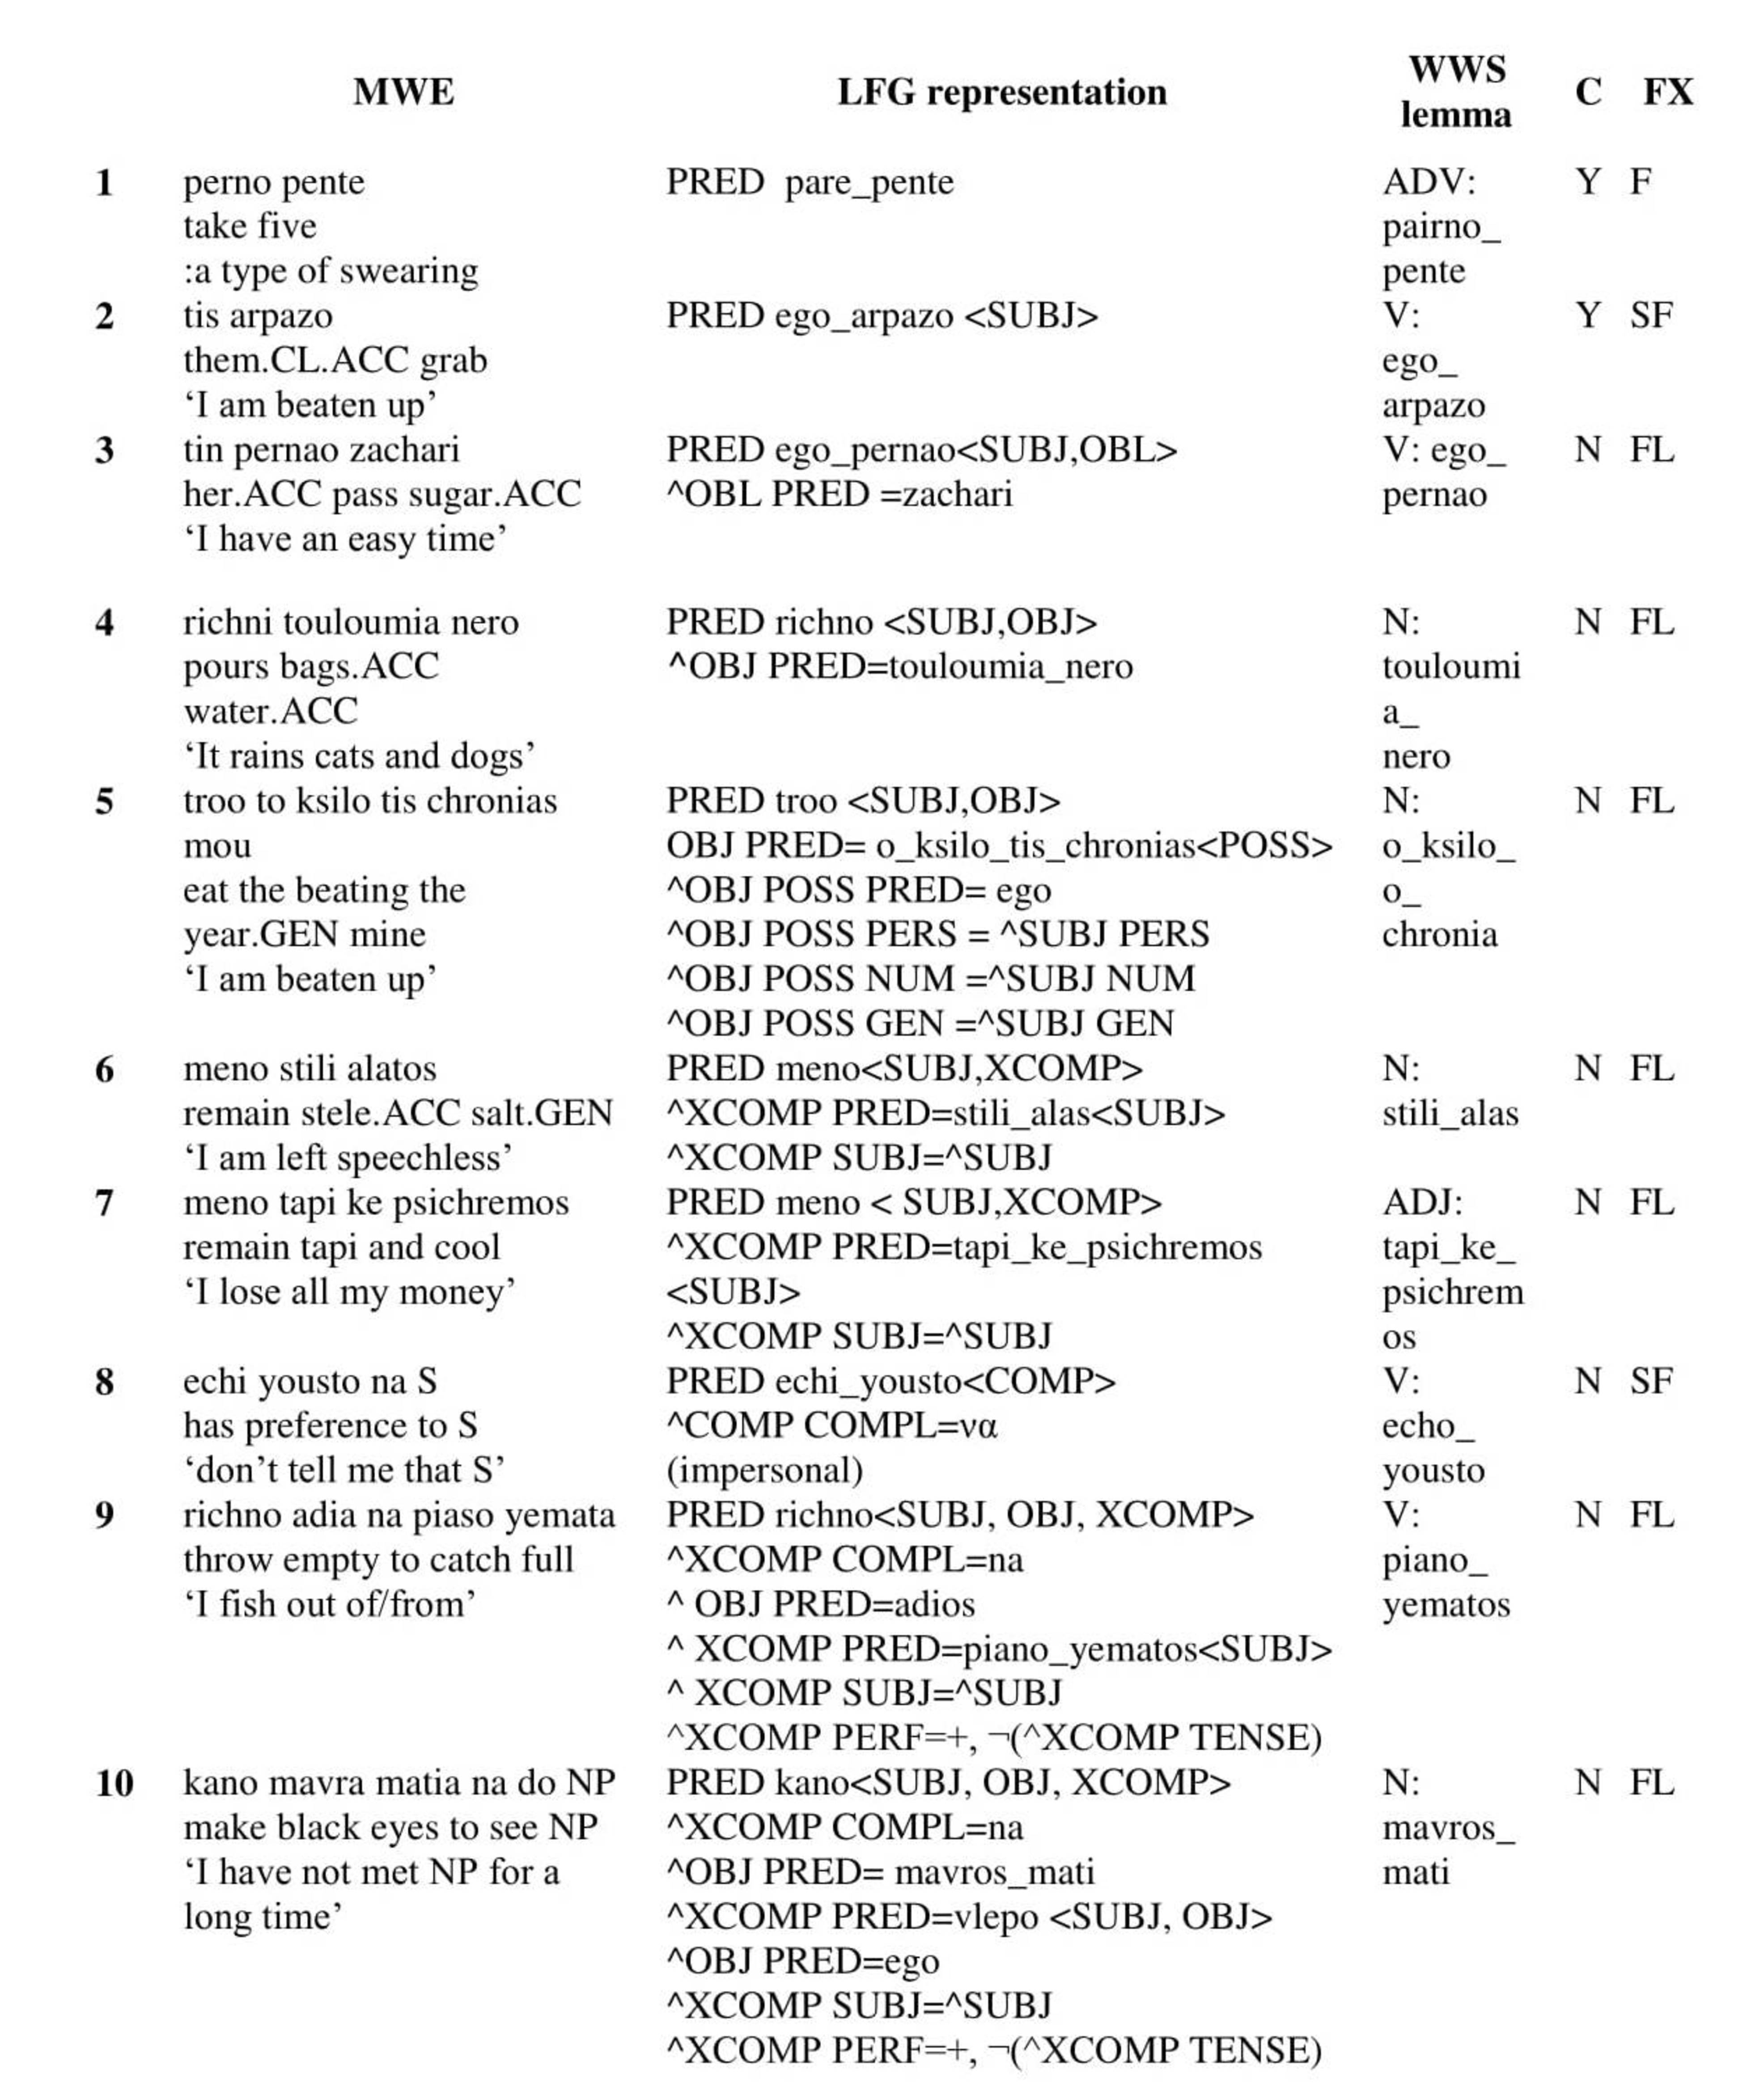
\includegraphics[width=1\textwidth]{figures/MWE_correct_table-1}
\resizebox{\textwidth}{!}{%
\begin{tabular}{l@{~}p{5.6cm}p{6.4cm}p{3.3cm}ll}
  %\hline
  \lsptoprule
  &  \textnormal{MWE} & \textnormal{LFG representation} & \textnormal{WWS lemma} & \textnormal{C} & \textnormal{FX} \\
  %\hline
  %\hline
  \midrule
  \textbf{1}
  &
  perno pente \newline
  take five \newline
  :a type of swearing
  &
  PRED pare\_pente 
  &
  ADV: \newline
  perno\_pente
  &
  Y
  &
  F
  \\
  \midrule
  \textbf{2}
  &
  tis arpazo \newline
  them.CL.ACC grab \newline
  `I am beaten up’
  &
  PRED ego\_arpazo <SUBJ>
  &
  V: \newline
  ego\_arpazo
  &
  Y
  &
  SF
  \\
  \midrule
  \textbf{3}
  &
  tin pernao zachari \newline
  her.ACC pass sugar.ACC \newline
  ‘I have an easy time’
  &
  PRED ego\_pernao <SUBJ,OBL> \newline
  $\uparrow$OBL PRED =zachari
  &
  V: \newline
  ego\_pernao
  &
  N
  &
  FL
  \\
  \midrule
  \textbf{4}
  &
  richni touloumia nero \newline
  pours bags.ACC water.ACC \newline
  `It rains cats and dogs’
  &
  PRED richno <SUBJ,OBJ> \newline
  $\uparrow$OBJ PRED=touloumia\_nero
  &
  N: \newline
  touloumia\_nero
  &
  N
  &
  FL
  \\
  \midrule
  \textbf{5}
  &
  troo to ksilo tis chronias mou \newline
  eat the beating the year.GEN mine \newline
  `I am beaten up’
  &
  PRED troo <SUBJ,OBJ> \newline
  OBJ PRED=o\_ksilo\_tis\_chronias<POSS>  \newline
  $\uparrow$OBJ POSS PRED= ego \newline
  $\uparrow$OBJ POSS PERS =$\uparrow$SUBJ PERS \newline
  $\uparrow$OBJ POSS NUM =$\uparrow$SUBJ NUM \newline
  $\uparrow$OBJ POSS GEN =$\uparrow$SUBJ GEN
  &
  N: \newline
  o\_ksilo\_o\_chronia
  &
  N
  &
  FL
  \\
  \midrule
  \textbf{6}
  &
  meno stili alatos \newline
  remain stele.ACC salt.GEN \newline
  `I am left speechless’
  &
  PRED meno <SUBJ,XCOMP> \newline
  $\uparrow$XCOMP PRED=stili\_alas<SUBJ> \newline
  $\uparrow$XCOMP SUBJ=$\uparrow$SUBJ
  &
  N: \newline
  stili\_alas
  &
  N
  &
  FL
  \\
  \midrule
  \textbf{7}
  &
  meno tapi ke psichremos \newline
  remain tapi and cool \newline
  `I lose all my money’
  &
  PRED meno <SUBJ,XCOMP> \newline
  $\uparrow$XCOMP PRED=tapi\_ke\_psichremos \newline
  <SUBJ> \newline
  $\uparrow$XCOMP SUBJ=$\uparrow$SUBJ
  &
  ADJ: \newline
  tapi\_ke\_psichremos
  &
  N
  &
  FL
  \\
  \midrule
  \textbf{8}
  &
  echi yousto na S \newline
  has preference to S \newline
  `don’t tell me that S’
  &
  PRED echi\_yousto <COMP> \newline
  $\uparrow$COMP COMPL=να \newline
  (impersonal)
  &
  V: \newline
  echo\_yousto
  &
  N
  &
  SF
  \\
  \midrule
  \textbf{9}
  &
  richno adia na piaso yemata \newline
  throw empty to catch full \newline
  `I fish out of/from’
  &
  PRED richno <SUBJ,OBJ,XCOMP> \newline
  $\uparrow$XCOMP COMPL=na \newline
  $\uparrow$OBJ PRED=adios \newline
  $\uparrow$XCOMP PRED=piano\_yematos<SUBJ> \newline
  $\uparrow$XCOMP SUBJ=$\uparrow$SUBJ \newline
  $\uparrow$XCOMP PERF=+, $\neg$($\uparrow$XCOMP TENSE) 
  &
  V: \newline
  piano\_yematos
  &
  N
  &
  FL
  \\
  \midrule
  \textbf{10}
  &
  kano mavra matia na do NP \newline
  make black eyes to see NP \newline
  `I have not met NP for a long time’
  &
  PRED kano <SUBJ,OBJ,XCOMP> \newline
  $\uparrow$XCOMP COMPL=na \newline
  $\uparrow$OBJ PRED= mavros\_mati \newline
  $\uparrow$XCOMP PRED=vlepo <SUBJ, OBJ> \newline
  $\uparrow$OBJ PRED=ego \newline
  $\uparrow$XCOMP SUBJ=$\uparrow$SUBJ \newline
  $\uparrow$XCOMP PERF=+, $\neg$($\uparrow$XCOMP TENSE)
  &
  N: \newline
  mavros\_mati
  &
  N
  & 
  FL
  %\\
  %\midrule
  \tabularnewline
  \lspbottomrule
\end{tabular}
}
\end{table}
A wide variety of structures is shown in Table~\ref{mar:types}. \textbf{1} is a sentence but functions as an adverb, the MWE in \textbf{2} and \textbf{3} function as intransitive verbs, \textbf{4} and \textbf{5} function as transitive verbs with \textbf{5} featuring a case of where the subject binds a possessive selected by the fixed object. \textbf{6} and \textbf{7} are predicative structures that contain a controlled adjectival constituent normally modeled as an XCOMP in \isi{LFG}. \textbf{8}, \textbf{9} and \textbf{10} are MWEs that contain sentential complements, either free (8) or subject to constraints such as control \textbf{9}, \textbf{10} and strong selection requirements on the form of the subordinated verb. These structures capture the typology of the 850 verb MWEs that we parsed. 
Below we give selected parse-outs of the material in Table~\ref{mar:types}. Please notice that all f-structures contain a sentential feature IDIOM that is of semantic nature and conveys the meaning of the MWE.
Figure~\ref{mar:Sfig5} shows the f-structure of (\ref{mar:ksilo xronias me ipok}) that features the verb MWE \textbf{5} in Table~\ref{mar:types}. This MWE contains an OBJ \isi{GF} headed by a WWS and a possessive anaphor that is analysed as a specifier of  the projection of the WWS and is bound by the free subject; as a result the free subject and the anaphor are of the same gender and number.  

 \ea\label{mar:ksilo xronias me ipok}
\gll	I Maria     efage to   ksilo      tis          chronias    tis \\
the Maria.\textsc{3sg}.\textsc{fem} ate the beating the year hers.\textsc{3sg}.\textsc{fem} \\
\glt `Maria was beaten up.’
\z

\begin{figure}[h!]
 \caption{\label{mar:Sfig5}f-structure for \textit{I Maria efage to ksilo tis chronias tis.} `Maria was beaten up.', example (\ref{mar:ksilo xronias me ipok}), MWE \textbf{5} in Table~\ref{mar:types}}
 \centering
 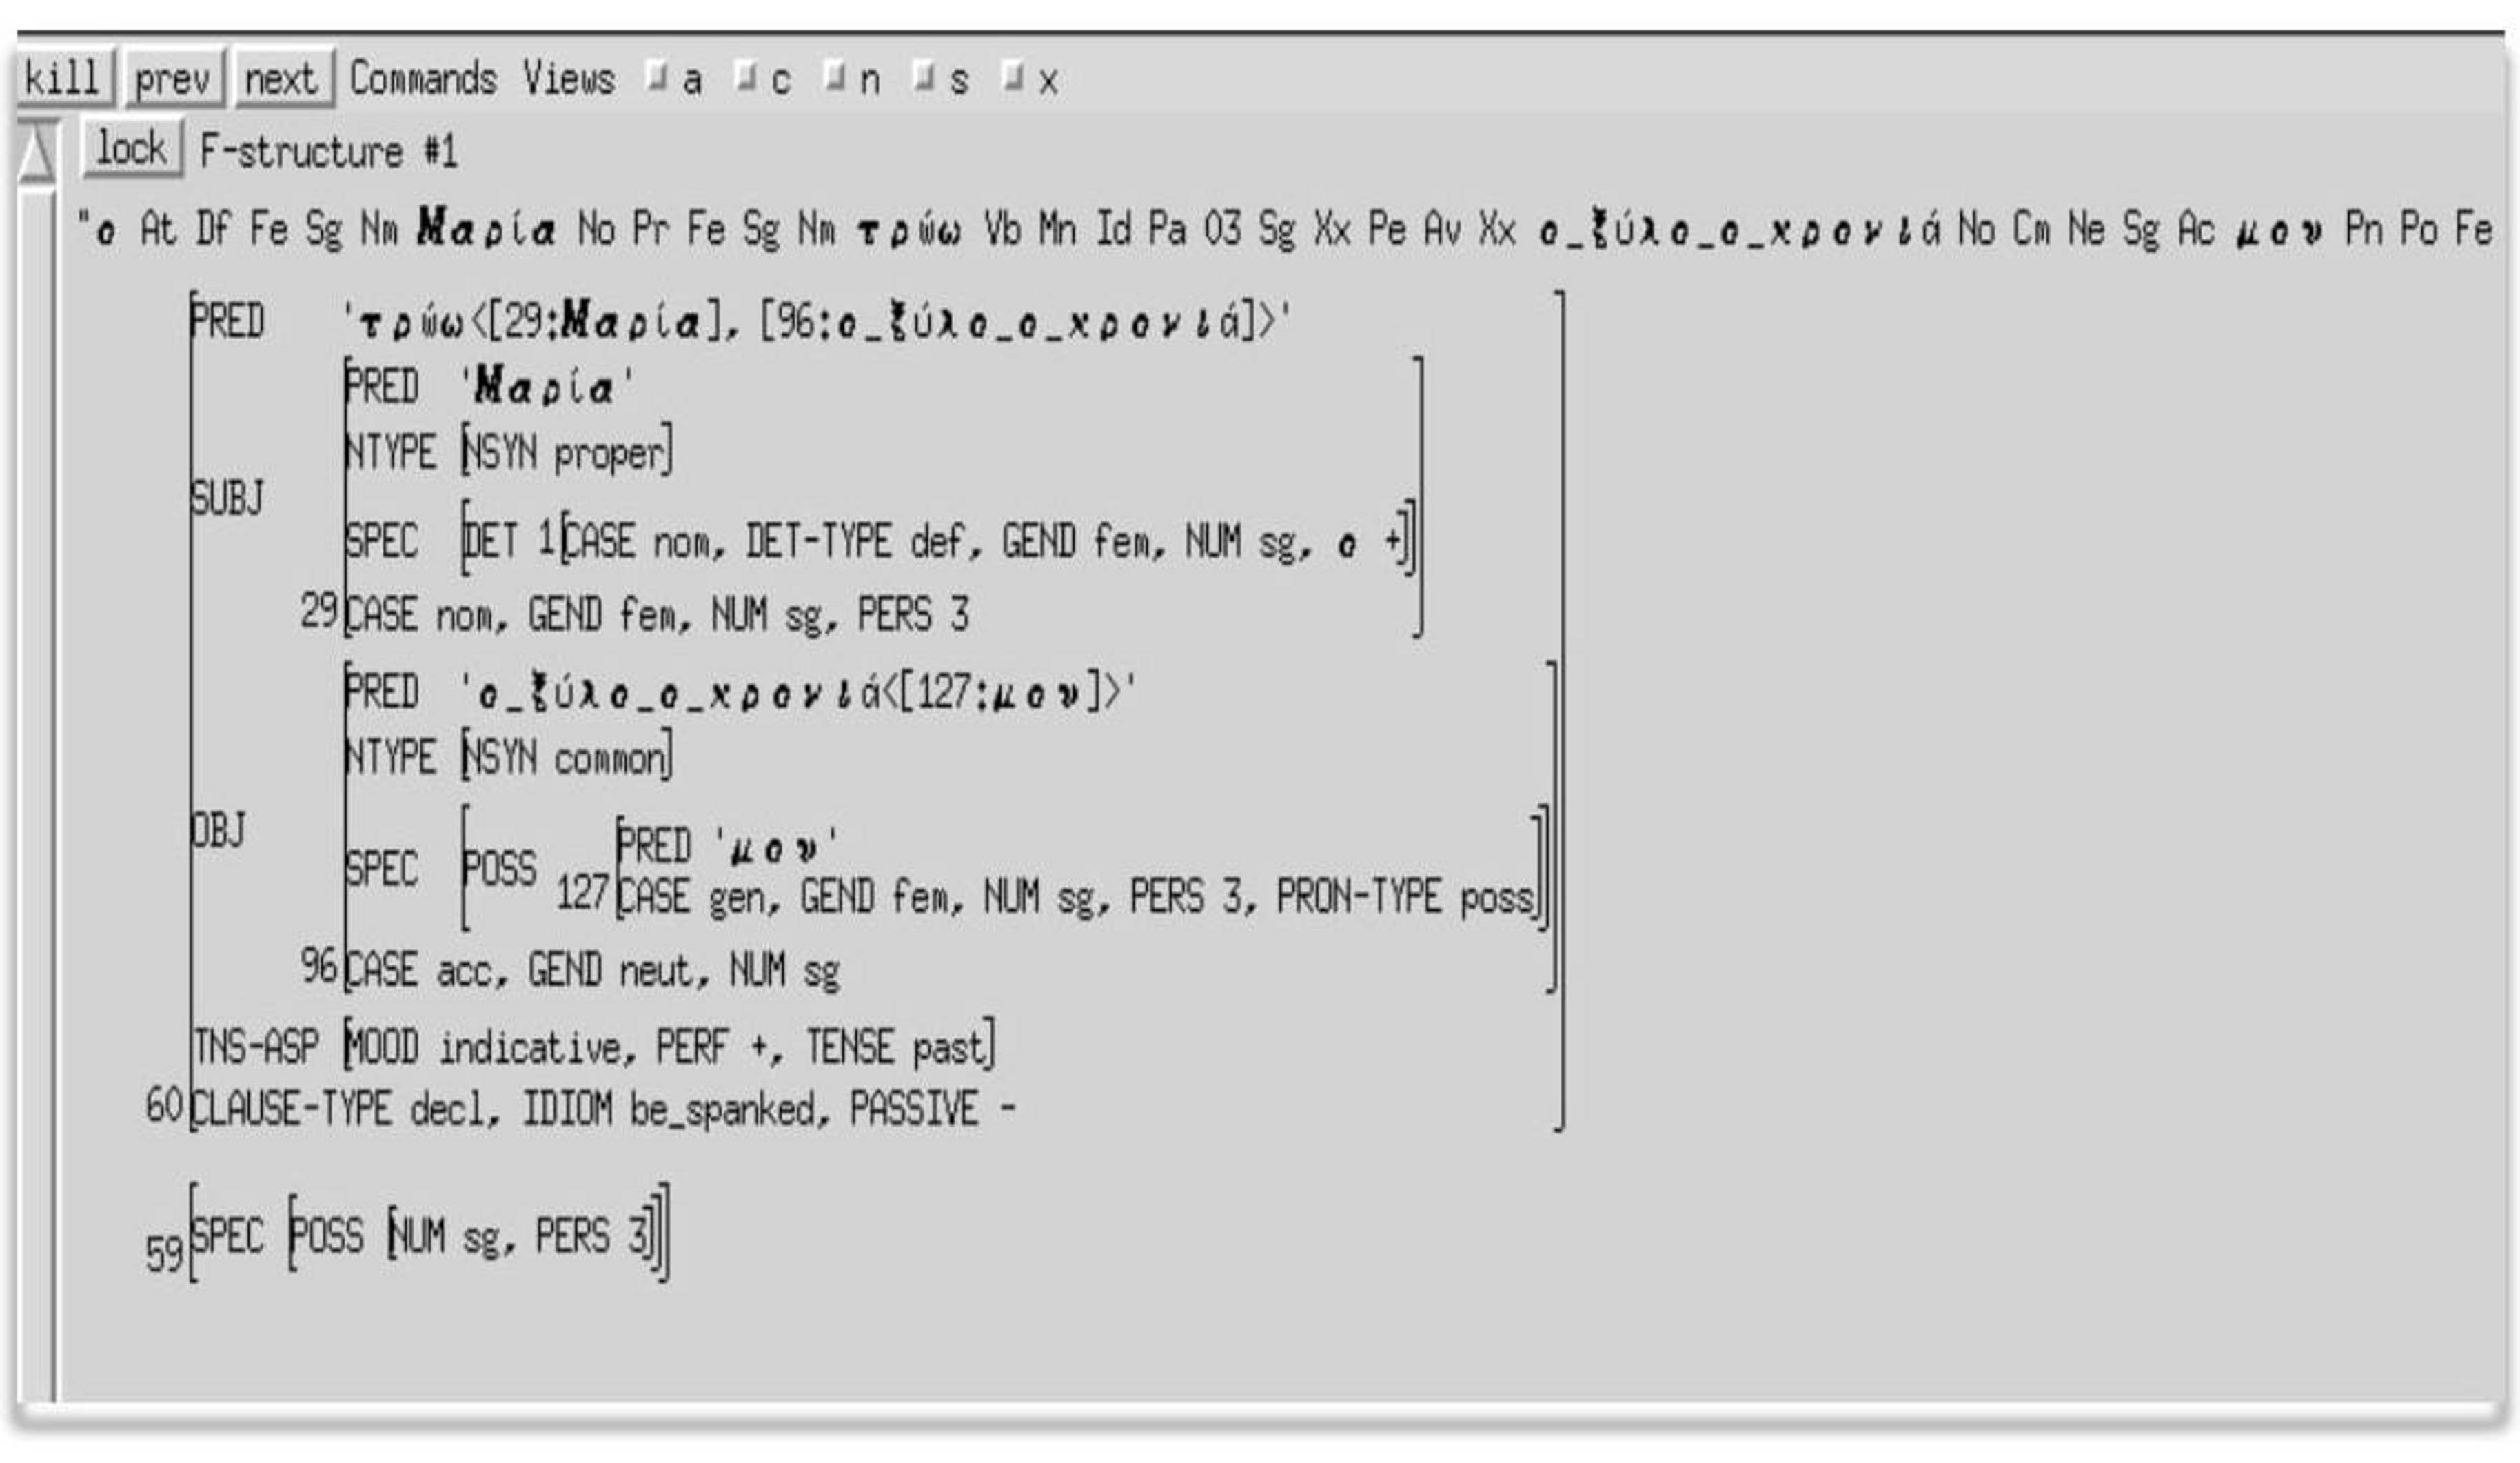
\includegraphics[width=1\textwidth]{figures/example9a}
 \end{figure}


Figure~\ref{mar:Sfig6} shows the c- and the f-structure of (\ref{mar:mavra matia subj}) that features an example of use of the verb MWE \textbf{10} in Table~\ref{mar:types} and of example (\ref{mar:basicexample}) that  contains an OBJ \isi{GF} headed by a WWS and a controlled sentential complement, an XCOMP in \isi{LFG} terms. The result of the application of the sub-lexical rules is shown on the c-structure. 

 \ea\label{mar:mavra matia subj}
\gll Ekana           mavra    matia    na  tin   do.\\ 
made.\textsc{1sg}   black      eyes      to  her see.\textsc{1sg}\\
\glt `I have not seen her for a very long time.’
\z
 
 \begin{figure}[p]%h!]
 \caption{\label{mar:Sfig6}c- and f-structure for \textit{Ekana mavra matia na tin do.} `I have not seen her for a long time.', example (\ref{mar:mavra matia subj}), MWE \textbf{10} in Table~\ref{mar:types}}
 \centering
 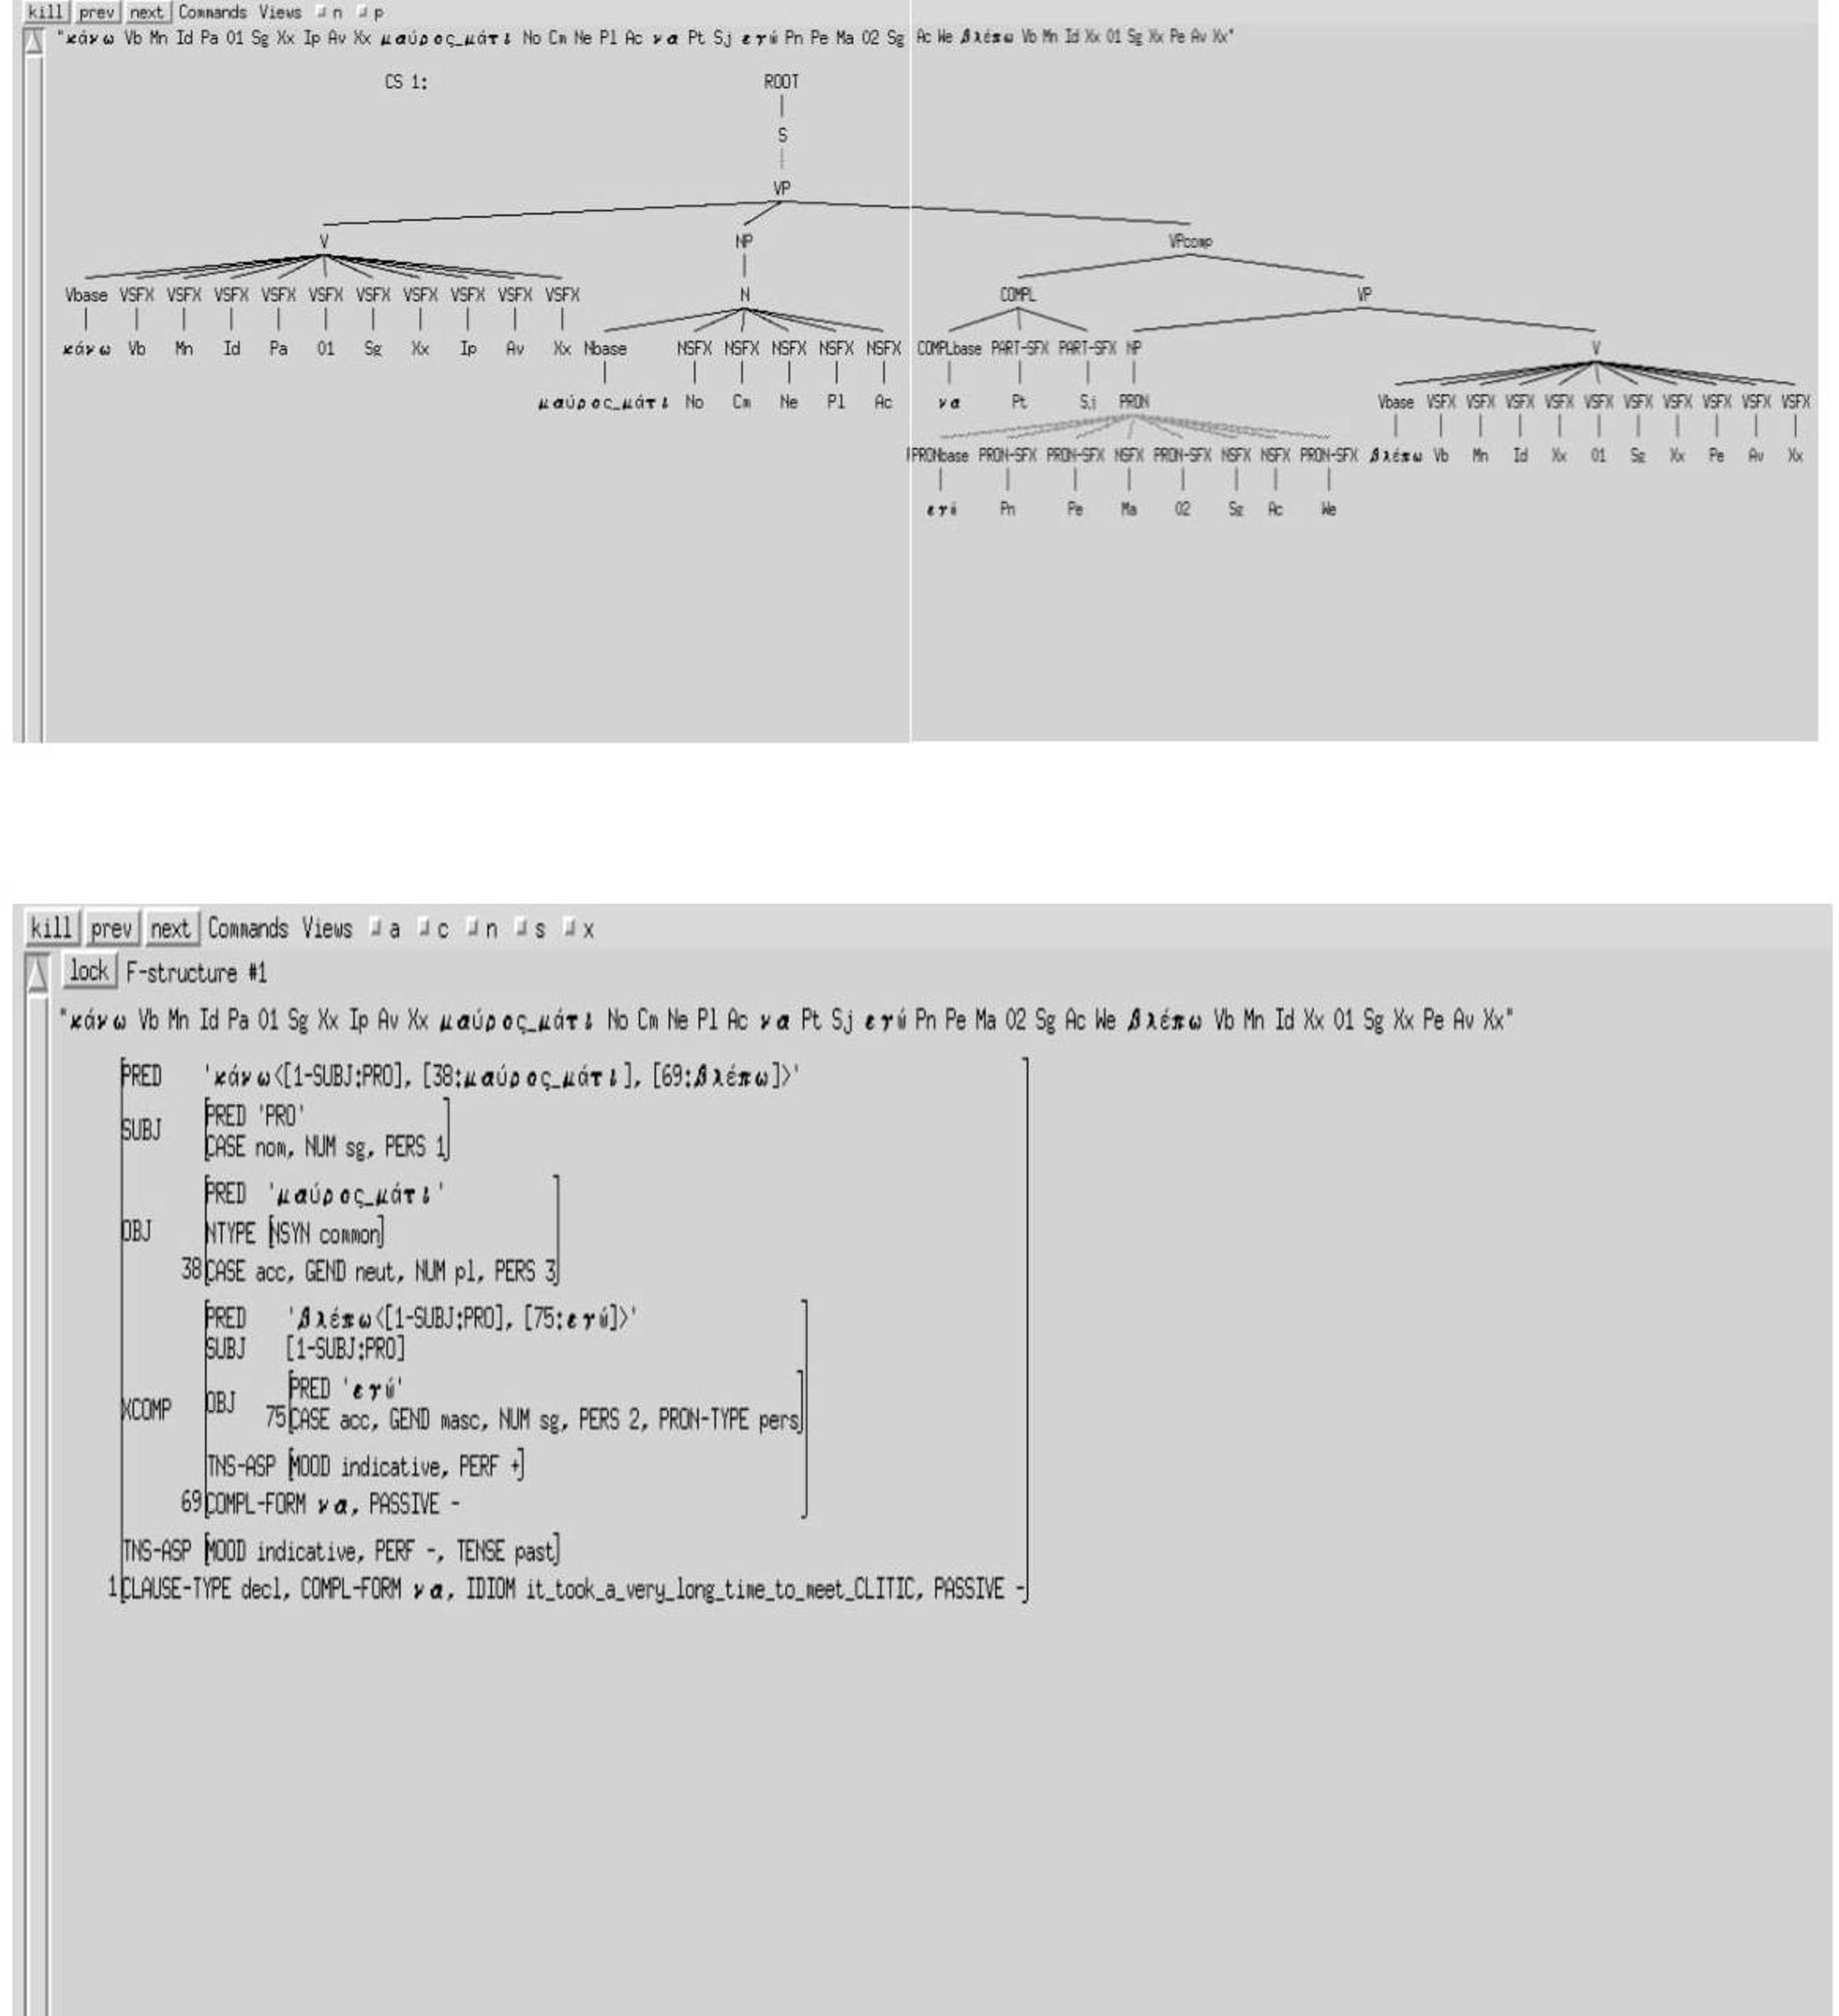
\includegraphics[width=1.\textwidth]{figures/example10a}
 \end{figure}
 

\section{Discussion}
We have presented a symbolic system for parsing MWEs that uses XLE and \isi{LFG} grammars as its main components. MWEs are recognized as such before entering the XLE component and their sequential fixed parts are processed to form words with spaces (WWS). WWSs are processed as words by the XLE component. This system definitely reduces ambiguity since fewer parsings are available by definition; furthermore, the system does not require a lexicon more elaborate than the one required by a ``compositional'' approach. However, we have no way to measure whether the system (with the components that have been implemented so far) performs faster as there is no base system that we can use for a comparison -- for instance, it would be interesting to evaluate the effect of the ambiguity that occurs in the filter. 

An interesting feature of the system presented here is that it receives lexical knowledge from a lexicographic resource (IDION) that has been developed independently. The embedding of IDION into the \isi{LFG}/XLE parsing system is a way of evaluating it. IDION has been designed with reusability issues in mind. However, the development of the transcription software indicated that some additional structural information would be beneficial, such as the marking of the head verbs and the marking of PPs (at the moment PPs are constructed by the transcription application that reads the IDION encoding and generates XLE entries). 
%
In the future, we aim to expand and improve the system in several ways, including an enrichment of IDION with other types of MWEs (nominal, adverbial), a more sufficient implementation of the filter and, of course, a \isi{grammar} capturing a wider range of MG structures. 

\section*{Abbreviations}
\begin{multicols}{2}
\begin{tabbing}
WWSs \hspace{1em} \= lexical functional grammar\kill
\isi{GF} \> grammatical function \\
\isi{LFG} \> lexical functional grammar \\
MG \> \ili{Modern Greek}  \\
NP \> noun \isi{phrase} \\
OBJ \> object \\
PoS \> part of speech \\
PP \> prepositional \isi{phrase} \\
SUBJ \> subject \\
WWSs \> words with spaces \\
\end{tabbing}
\end{multicols}

%IDION http://idion.ilsp.gr
%ILSP FBT Tagger http://lrt.clarin.eu/tools/ilsp-feature-based-multi-tiered-pos-tagger
%ILSP-PAROLE compatible Tagset: http://nlp.ilsp.gr/nlp/tagset_examples/tagset_en/index.html
%XLE documentantion http://www2.parc.com/isl/ groups/nltt/xle/doc/xle_toc.html

%References used for the development of the filter:
%http://www.it.uom.gr/project/perl/win32perltut.html
%https://www.perl.org/books/beginning-perl/
%https://qntm.org/files/perl/perl.html
%http://learn.perl.org/
%http://perldoc.perl.org/perlintro.html
%http://www.cs.tut.fi/~jkorpela/perl/regexp.html \end{verbatim}|

%Anastasiadi-Symenonidi, Anna. 1986. Neology in \ili{Modern Greek} Koine. Thessaloniki. EEFS of University of Thessaloniki, Anex 65.\\ 

%% REMOVED IN THE FINAL VERSION
%%\nocite{apidianaki2018,attia2006,bargmann2017,copestakeetal2002,crabbe:etal:13,dalrymplelfg,fotopoulou1993,gregoire:10,gross1988b,gross1988a,kay,korkontzelosetal2010,markantonatou2015,markantonatou2017,mini2011,minos2016,papageorgiou2000,pollard1994,przepiorkowski2014,sag02,samaridi2014,waszczuk2015}

%% \begin{thebibliography}{}
%% \bibitem{} Apidianaki, Marianna, Prokopis Prokopidis, and Haris Papageorgiou. 2018. Combining Cross-lingual and Syntactic Evidence for Greek MultiWord Expression Identification. In Stella Markantonatou and Anastasia Christofidou (eds). Special issue on MWEs in Greek and other languages: from theory to implementation, Bulletin of Scientific Terminology and Neologisms of the Academy of Athens, Athens, Greece.
%% \bibitem{} Attia, Mohammed A. 2006. Accommodating \isi{Multiword Expressions} in an \ili{Arabic} \isi{LFG} Grammar. Salakoski, Tapio, Ginter, Filip, Pahikkala, Tapio, Pyysalo, Tampo: Lecture Notes in Computer Science: Advances in Natural Language Processing, 5th International Conference, FinTAL. Turku, Finland. Vol. 4139. Springer-Verlag Berlin Heidelberg. 87-98.
%% \bibitem{} Bargmann, Sascha \& Manfred Sailer. 2017. The Syntactic Flexibility of Semantically Non-decomposable Idioms. In Manfred Sailer and Stella Markantonatou (eds). Mutliword Expressions: Insights from a Multi-lingual Perspective. Language Science Press.
%% \bibitem{} Copestake, Ann, Fabre Lambeau, Aline  Villavicencio, Francis Bond, Timothy Balwin, Ivan A. Sag, and Dan Flickinger. 2002. Multiword expressions: linguistic precision and reusability. Proceedings of the 3rd International Conference on Language Resources and Evaluation. Las Palmas, Canary Islands.
%% \bibitem{} Crabb\'e, Beno\^it, Denys Duchier, Claire Gardent, Joseph Le Roux, Yanick Parmentier. 2013. XMG: eXtensible MetaGrammar. Computational Linguistics 39 (3). MIT Press. 591-629.
%% \bibitem{} Dalrymple, Mary. 2001. Lexical Functional Grammar (Syntax and Semantics 34). CA: Academic Press.
%% \bibitem{} Fotopoulou, Aggeliki. 1993. Une Classification des Phrases a Complements Figés en Grec Moderne. Doctoral Thesis, Universite Paris VIII.
%% \bibitem{} Grégoire, Nicole. 2010. DuELME: a \ili{Dutch} electronic lexicon of multiword expressions. Language Resources and Evaluation 44.1-2. 23–39.
%% \bibitem{} Gross, Maurice. 1988a. Les limites de la \isi{phrase} figée. Langage 90. 7-23.
%% \bibitem{} Gross, Maurice. 1988b. Sur les phrases figées complexes du français. Langue française 77. 47-70.
%% \bibitem{} Kay, Paul \& Ivan A. Sag. 2012. A Lexical Theory of Phrasal Idioms. Unpublished manuscript. Stanford University. \url{http://www1.icsi.berkeley.edu/~kay/idioms-submitted.pdf}. A revised version is available at \url{http://www1.icsi.berkeley.edu/~kay/idiom-pdflatex.11-13-15.pdf}
%% \bibitem{} Korkontzelos, Ioannis \& Suresh Manandhar. 2010. Can Recognising \isi{Multiword Expressions} Improve Shallow Parsing? Human Language Technologies: The 2010 Annual Conference of the North American Chapter of the ACL, Los Angeles, California, June 2010. 636–644.
%% \bibitem{} Markantonatou, Stella \& Niki Samaridi. 2017. Verb MWEs and the grammatical function `object'. In Manfred Sailer \& Stella Markantonatou (eds). Mutliword Expressions: Insights from a Multi-lingual Perspective. Language Science Press.
%% \bibitem{} Markantonatou Stella, Eri Koletti, Elpi Margariti, Panagiotis Minos, Aimilia Stripeli, Giorgos Zakis and Niki Samaridi. 2015. Database for free subject verb MWEs.  PARSEME 4th general meeting in Valetta, Malta. \url{http://typo.uni-konstanz.de/parseme/ images/Meeting/2015-03-19-Malta-meeting/WG1-MARKANTO NATOU-ETAL-poster.pdf}
%% \bibitem{} Mini, Marianna, Kleopatra Diakogiorgi and Aggeliki Fotopoulou. 2011. What can children tell us about idiomatic phrases’ fixedness: the psycholinguistic relevance of a linguistic model. DISCOURS (Revue de linguistique, psycholinguistique et informatique) 9.
%% \bibitem{} Minos, Panagiotis, Stella Markantonatou, Georgios Zakis and Elpiniki Margariti. 2016. Generating \isi{LFG}/XLE MWE entries from IDION (a theory neutral lexical DB). Parseme 6th general meeting in Struga/fYROM. \url{http://typo.uni-konstanz.de/parseme/index.php/2-general/156-selected-posters-struga-7-8-april-2016}
%% \bibitem{} Papageorgiou, Haris, Prokopis Prokopidis, Voula Giouli and Stelios Piperidis. 2000. A Unified POS Tagging Architecture and its Application to Greek. Proceedings of the 2nd Language Resources and Evaluation Conference. Athens.
%% \bibitem{} Pollard, Carl \& Ivan A. Sag. 1994. Head Driven Phrase Structure Grammar. Chicago: University of Chicago Press.
%% \bibitem{} Przepiórkowski, Adam, Elzbieta Hajnicz, Agnieszka Patejuk and Marcin Woliński. 2014. Extended phraseological information in a valence dictionary for NLP applications. Proceedings of the workshop on lexical and grammatical resources for language processing (LG-LP 2014). 83–91. Dublin, Ireland.
%% \bibitem{} Sag, Ivan A., Timothy Baldwin, Francis Bond, Ann Copestake  and Dan Flickinger. 2002. \isi{Multiword Expressions}: A Pain in the Neck for NLP. LinGO Working Paper No. 2001-03. In Alexander Gelbukh, ed., (2002) Proceedings of CICLING-2002. Springer-Verlag Berlin Heidelberg.
%% \bibitem{} Samaridi, Niki \& Stella Markantonatou. 2014. Parsing \ili{Modern Greek} verb MWEs with \isi{LFG}/XLE grammars. The 10th Workshop on \isi{Multiword Expressions} (MWE 2014), Workshop at EACL 2014 (Gothenburg, Sweden), April 26-27, 2014.
%% \bibitem{} Waszczuk, Jakub \& Agata Savary. 2015. "Modeling syntactic properties of MWEs in \isi{LFG}" PARSEME's 4th general meeting in Valletta, Malta 19-20 March 2015.
%% \end{thebibliography}

\printbibliography[heading=subbibliography,notkeyword=this]

\end{document}
